\subsection{Experiment 7: Scaling Complexity} \label{sec:exp7}

Building upon the success of the previous experiment, the purpose of this study was to replicate the same approach utilizing larger models. This was achieved by amplifying the number of convolutional layers in each block and the number of filters in each convolutional layer.

This experiment tested two sets of models. The first set comprised of models, each with 10 million parameters, resulting in a total of 20 million parameters. The second set includes models with a total of 50 million parameters, each having 25 million parameters.

The other configuration aspects, such as the loss function, regularization techniques, data set, optimizer, and hardware configuration, remained the same.

In the initial test, the generator loss of $1.132$ and the discriminator loss of $1.389$ resulted in a total loss of $2.512$.

For a visual representation of the experiment results, including the loss and final spectrogram, please see Figure~\ref{fig:exp7_10_results}.

\begin{figure}[!ht]
    \centering
    \begin{subfigure}{0.45\textwidth}
        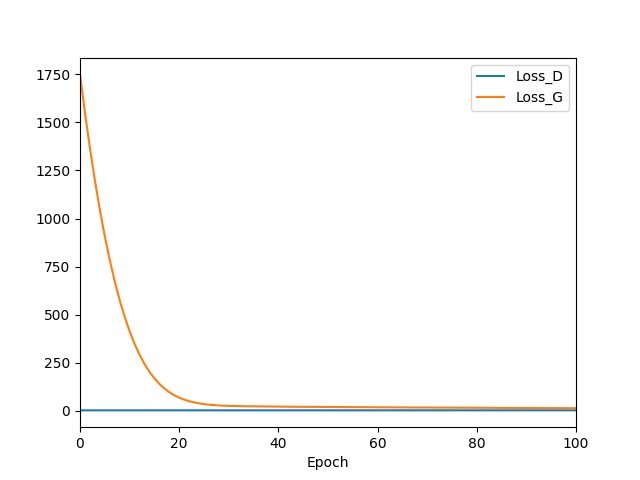
\includegraphics[width=\textwidth]{figures/4.5-results/exp7_10_loss.png}
        \caption{Evolving losses throughout the training process for Experiment 7 with 20 million parameters.}
        \label{fig:exp7_10_loss}
    \end{subfigure}
    \begin{subfigure}{0.45\textwidth}
        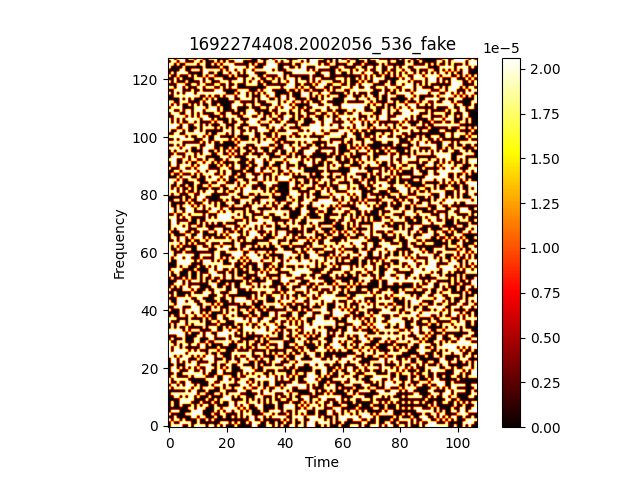
\includegraphics[width=\textwidth]{figures/4.5-results/exp7_10_spectrogram.png}
        \caption{Spectrogram generated in Experiment 7 with 20 million parameters.}
        \label{fig:exp7_10_spectrogram}
    \end{subfigure}
    \caption{Results of Experiment 7 with 20 million parameters.}
    \label{fig:exp7_10_results}
\end{figure}

The second experiment resulted in a total loss of $3.177$, comprising a generator loss of $1.738$ and a discriminator loss of $1.439$.

To view the experiment results, including the loss and final spectrogram, refer to Figure~\ref{fig:exp7_25_results}.

\begin{figure}[!ht]
    \centering
    \begin{subfigure}{0.45\textwidth}
        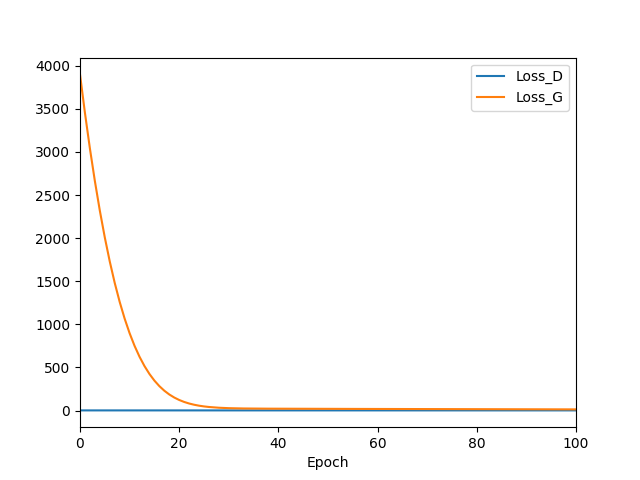
\includegraphics[width=\textwidth]{figures/4.5-results/exp7_25_loss.png}
        \caption{Evolving losses throughout the training process for Experiment 7 with 50 million parameters.}
        \label{fig:exp7_25_loss}
    \end{subfigure}
    \begin{subfigure}{0.45\textwidth}
        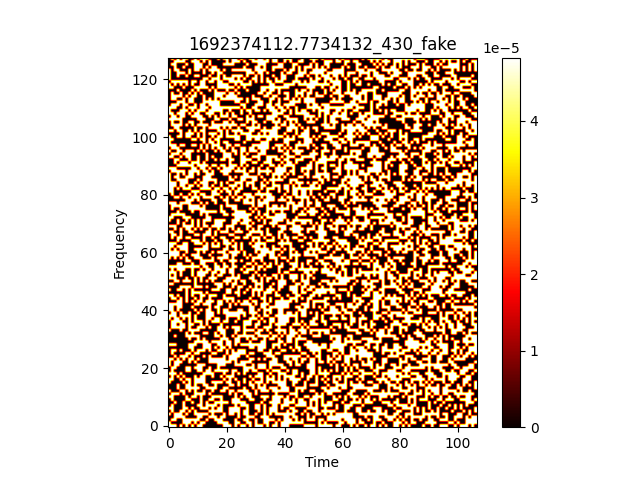
\includegraphics[width=\textwidth]{figures/4.5-results/exp7_25_spectrogram.png}
        \caption{Spectrogram generated in Experiment 7 with 50 million parameters.}
        \label{fig:exp7_25_spectrogram}
    \end{subfigure}
    \caption{Results of Experiment 7 with 50 million parameters.}
    \label{fig:exp7_25_results}
\end{figure}

